
\section{Ausrichtung des Solarpanels}\label{sec:ausrichtung des Solarpanels}
Um die Leistungsaufnahme des Solarpanels zu optimieren ist es notwendig dieses direkt auf die Sonne auszurichten und diese Ausrichtung auch in geeigneten Zeitabständen zu korrigieren. Im Vergleich mit einem fest ausgerichteten Solarpanel konnten J. Rizek \emph{et al.} mit einem nachgeführten Solarpanel beispielsweise die Leistungsaufnahme um durchschnittlich 30\% erhöhen~\cite{Rizek2008}.

Hierfür kommen grundsätzlich verschiedene Methoden in Frage. In diesen Fall soll die Position der Sonne relativ zur Wetterstation auf Grundlage des Längen- und Breitengrades, der Uhrzeit und des Kalendertages berechnet werden. Diese Information werden über das GPS-Modul bereitgestellt. Anschließend wird das Solarpanel mit Hilfe der Motoren, des Kompass-Moduls und des am Panel befestigten Neigungssensors auf die Sonne ausgerichtet.

\subsection{Berechnung der Sonnenposition}\label{sec:berechnung_der_sonnenposition}
Da die Formeln zur Berechnung der Sonnenposition in diesem Projekt lediglich benutzt werden, wird an dieser Stelle auf eine Herleitung verzichtet. Die verwendeten Formeln können beispielsweise im \emph{Astronomical Almanac}~\cite{Anon1984} gefunden werden. \emph{M. L. Roderick} beschreibt die nötigen Berechnungen in seinem Report~\cite{Roderick1992} und liefert zudem compilierbaren C-Code. Dieser wird im folgenden zur Berechnung der Sonnenposition verwendet.

Die Position der Sonne, im Bezug auf einen Beobachter auf der Erde, lässt sich durch die Werte \emph{Zenith} und \emph{Azimut} eindeutig beschreiben. Der Zenith beschreibt den Winkel zwischen einer Linie vom Beobachter zur Sonne und der Vertikalen. Der Azimut den Winkel zwischen der Horizontalen und Norden. Dabei stehen beispielsweise ein Azimut von \SI{90}{\degree} für Osten, \SI{180}{\degree} für Süden und \SI{270}{\degree} für Westen. Eine Veranschaulichung kann in Abbildung~\ref{fig:zen_azi} gefunden werden.

\begin{figure}[H]
  \centering
  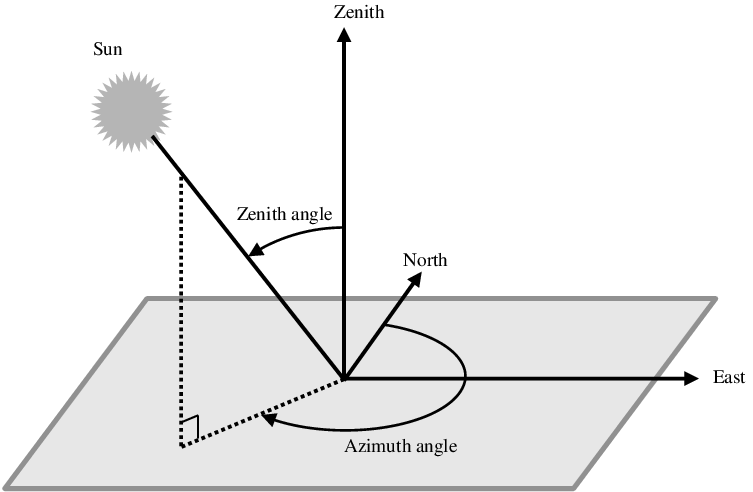
\includegraphics[width=\textwidth]{./img/Representation-of-azimuth-and-zenith-angles.png}
  \caption{Beschreibung der Sonnenposition durch Zenith und Azimut~\cite{Nou2016}}\label{fig:zen_azi}
\end{figure}

Die Genauigkeit der verwendeten Formeln beträgt laut dem \emph{Astronomical Almanac} \SI{0.01}{\degree} bezogen die auf die Position und \SI{0.1}{\minute} bezogen auf die Zeit.


%%% Local Variables:
%%% mode: latex
%%% TeX-master: "../termpaper"
%%% End:
